\section{Long period comparison}
\label{sect:lts_study}
Aim is to test a series of ODS with different selection, scoring and biasing then some basic LAS with different placement heuristics over a period of 2 months (2 lunar cycles) to determine tendencies. The following schedulers/components are to be used:-

\begin{itemize}
\item BDS using standard HSMs and best selection model $\zeta_{best}$.
\item BDS using biased selection models i.e fixed rank bias $\zeta_{fr}$ and relative score bias $\zeta_{rs}$.
\item BDS using biasing and rank-ordered metric selection
\item Simple LAS and test various placement strategies.
\end{itemize}

What results do I expect from the 3 first models? - Running with fixed env to eliminate some random variation, still have stochastic exec timing variation. Fixed phase2model - see shakedown to see how this effects error bars - will test variation of phase2 (Load/contention) as variation parameter later series of experiments.

So far we have been looking simple simulations with fixed E,P models and allowing the only source of random variation to be the SEM. Operationally it is found that the actual exec times of groups is modelled reasonably well by the Exec timing model so this would infact account for a small effect.

We now wish to see how effective the various schedulers are under varying P and E models. In particular we would like to be able to obtain a single characteristic for a P or E model which would allow us to plot scheduler  SQMs against these characteristics.

In reality to fully describe an E or P model requires a number (in the case of P, a very large number) of parameters. We therefore seek to find a single charcateristic which can be measured for these models and thus sued a s an independant variable.

From a defined set of E model parameters we can generate any number of E scenarios (effectively instantiations of the model) - it would be useful to see if we get variation in results and indeed in the ``measured characteristic'' (SQMs) from different scenarios generated by the same model - if this variation is large we will have to run many more simulations and there will be x-errors in addition to the expected y-errors.

A similar situation occurs with P models - we can generate many P scenarios (instantitations) from a single set of P model parameters - and hence probably different ``measured characteristics''.

We need to check the stability of characteristics for initial model parameters.

\subsection{Check variation of environment model characteristics}

Using an Env model generator with stability parameter tau such that the seeing remains in a stable state for a period averaging around tau. The seeing scenario is generated by taking random intervals calculated from $-\tau_e \ln{(1-R)}$ where R is a random number in $[0,1]$. At each period the seeing changes randomly to another value - we are not bothered which value or how the seeing states are distributed only that it is changing. Results of a run with $\tau_e =30 mins$ are shown in Fig.~\ref{fig:env_profile_18} which shows the actual seeing scenario over a period of 7 days. Fig.~\ref{fig:env_comp_18} shows a comparison for the relative amounts of time under varying lengths of stability period for several runs of the $E_{1800}$ model. We see from this that the models are generally quite stable i.e. that a given control parameter $\tau_e$ gives consistent results in terms of the distribution of lengths of stable periods. Fig.~\ref{fig:env_relstats} and  Fig.~\ref{fig:env_cumstats} show the relative and cumulative distribution of lengths of periods of stability for various models with $\tau_e$ running from 30 minutes to 4 hours over scenario runs of 100 days.

\begin{figure}[h]
\begin{center}
 \includegraphics[scale=0.5, angle=-90]{figures/e_18_prof.eps}
\end{center} 
 \caption[Environmental scenario (7 day snapshot).] 
   {Long period study. 7 day snapshot of generated environmental scenario $E_{1800}$.}
\label{fig:env_profile_18}
\end{figure}


\begin{figure}[h]
\begin{center}
 \includegraphics[scale=0.5, angle=-90]{figures/e_18_comp.eps}
 \caption[Environmental scenario - comparison between runs of $E_{1800}$] 
   {Long period study. Comparison of relative amounts of time in periods of stability for several runs of $E_{1800}$.}
\end{center} 
\label{fig:env_comp_18}
\end{figure}

\begin{figure}[h]
\begin{center}
 \includegraphics[scale=0.5, angle=-90]{figures/e_relstats.eps}
 \caption[Environmental scenario - relative distribution of stable period lengths.] 
   {Long period study. Relative distribution - number of periods with stability in variable range.}
\end{center} 
\label{fig:env_relstats}
\end{figure}

\begin{figure}[h]
\begin{center}
 \includegraphics[scale=0.5, angle=-90]{figures/e_cumstats.eps}
 \caption[Environmental scenario - cumulative distribution of stable period lengths.] 
   {Long period study. Cumulative distribution - total time where stability upto variable range.}
\end{center} 
\label{fig:env_cumstats}
\end{figure}

\begin{itemize}
\item each sim will use 100-1000 runs - get back graphs of: distibution of qsu for a single night, ensemble plot of qsu over time to show day to day variation and randomness. averagae and stdev for qsu.
\item another sim will show effect of varying DE the env stability parameter - plot each zetamodel as seperate graph with errorbars
\item another sim will show effect of varying DB - ie mean contention as ODB size characteristic - diff plots per zetamodel
\end{itemize}


Later we will fiddle with these and use different types of E and W prediction models (ie with different accuracy though not real models.) to see what works best under different scenarios - i.e want to test these under varying scenario parameter as independant variable(s).

Figure \ref{fig:env_snap_1} shows a snapshot of the environmental (seeing) scenario used for this study. It consists of some 1800 seeing category changes over the 60 day period (average duration 48 minutes) with individual durations taken from the seeing model described in table \ref{tab:ltc_env_scenario} and photometric/spectrometric extinction ratio set to 4\:1.

\begin{figure}[h]
\begin{center}
 \includegraphics[scale=0.5, angle=-90]{figures/env_snapshot_2007-11-15_72.eps}
 \caption[Environmental scenario 2007-11-15 (72 hour snapshot).] 
   {Long period study. Snapshot of environmental scenario.}
\end{center} 
\label{fig:env_snap_1}
\end{figure}

\begin{table}[h]
 \label{tab:ltc_env_scenario}
 \begin{center}
  \begin{tabular}{lllll}
   \toprule
   \multicolumn{4}{c}{Environmental scenario parameters} \\
   \midrule
   Seeing class & $\mu$ & $\sigma$ & min \\
   \midrule
   \emph{Excellent} & 0.5 & 0.25  & 0.05 \\
   \emph{Average}   & 1.0 & 0.5   & 0.05 \\
   \emph{Poor}      & 1.0 & 0.25  & 0.1 \\
   \emph{Unusable}  & 0.2 & 0.025 & 0.05 \\
   \bottomrule
  \end{tabular}
 \end{center}
\caption{Details of seeing component of environmental scenario generator model.} 
\end{table}


Need some graphs showing various examples of env stability models as actual seeing wrt time - ie how does the DE parameters make the seeing graph actually look - it is a param which shows how stable the env is to changes up or down - effectively how long it stays in any state see figs ($env_stab_de_xx, env_stab_de_yy, zz$ where xyz are de values in hours).

Here is the general E model specification

\[ \left( 
\begin{array}{ccc}
  P_{11}(t) & P_{12}(t) & P_{13}(t) \\
  P_{21}(t) & P_{22}(t) & P_{23}(t) \\
  P_{31}(t) & P_{32}(t) & P_{33}(t) 
\end{array} 
\right)\] 

\subsection{Check variation of Phase2 model characteristics for generated models}

Before we start need some idea of what sort of P2M to use - real or generated. A real model suffers from the ODB evolution problem (see \ref{XXX}). With a generated P2 model, group activations are spread out over a specified period (say several months) so new groups are appearing in the schedule every day - like the real ODB but in that case they are not entered until required so we dont know about them in advance and cannot take them into account easily.
   
 First set up a few generated P2 models and run some tests - basically use a simple BDS with a fixed environmental scenario and see how some easily calculated and visualized PCM looks - the daily average value of the dynamic contention profile $C_{DC}$ is chosen as it is easily visualized. These tests are all run from 15-oct-07 to 15-dec-07 and have different levels of contention. Table \ref{tab:ltc_p2models} shows details of the phase2 models tested.

\begin{table}[h]
\label{tab:ltc_p2models}
 \begin{center}
  \begin{tabular}{lllll}
   \toprule
   \multicolumn{5}{c}{Phase2 models - more detail required} \\
   \midrule
   DBID & ODB Date & CPlot & NPlot & Description\\
   \midrule
   $P_s$ & 22nov07 midpoint & c1 & p1 & P2Gen small model \\ 
   $P_l$ & 22nov07 midpoint & c3 & p3 & P2Gen light model \\
   $P_m$ & 22nov07 midpoint & c3 & p3 & P2Gen medium model\\
   $P_h$ & 22nov07 midpoint & c2 & p2 & P2Gen heavy model \\
   \midrule
   $O_1$ & 15oct07 snapshot & c4 & p4 & ODB Day 0 Snapshot\\
   $O_2$ & 25sep07 snapshot & c5 & p5 & ODB -20 day snapshot\\
   \bottomrule
  \end{tabular}
 \end{center}
\caption{Phase2 model descriptions - need more info on these than what is in table esp the gen models}
\end{table}

Results for 4 generated models $P_l$ - $P_h$ are shown in figures \ref{fig:c60_gen_av} and \ref{fig:c60_gen_ng}. Similar figures for the ODB snapshots though on a different scale (what does that mean?) are shown in \ref{fig:c60_odb_av} and \ref{fig:c60_odb_ng}.

\begin{figure}[h]
\begin{center}
 \subfigure[Variation of average contention $\bar{C_c}$ for generated phase2 models.] {
   \label{fig:c60_gen_av}
   \includegraphics[scale=0.25, angle=-90]{figures/c60_gen_cav.eps}
  }
 \subfigure[Variation of number of executed groups for generated phase2 models.] {
   \label{fig:c60_gen_ng}
   \includegraphics[scale=0.25, angle=-90]{figures/c60_gen_ng.eps}
  }
 \subfigure[Variation of average contention $\bar{C_c}$ for ODB snapshots.] {
   \label{fig:c60_odb_av}
   \includegraphics[scale=0.25, angle=-90]{figures/c60_odb_cav.eps}
  }
 \subfigure[Variation of number of executed groups for ODB snapshots.] {
   \label{fig:c60_odb_ng}
   \includegraphics[scale=0.25, angle=-90]{figures/c60_odb_ng.eps}
  }
\caption{Comparison of average contention measure and number of groups executed per night for generated phase2 models and ODB snapshots.}
 \end{center}
\end{figure}

From a given generator model (e.g. $P_l$) we can generate any number of actual instances - ideally these would all have the same measurable characteristics (e.g. $\bar{C_c}$) but this is not guaranteed. Tests were run using each of the generator models in order to determine the variation of characteristics. The measurable characteristic chosen was $\bar{C_{dc}}$ - the average dynamic contention over the measurment period. A simple scheduler was chosen using best-score selection and a single $f_{OH}$ metric - i.e. the target which was highest relative to maximum attainable elevation was chosen at each sweep. We are not interested in the scheduler here, only the variability of the generated  P2 characteristics. Simulations were run for the middle 30 days () of the generated models and the values of $\bar{Q_{SU}}$ and $\bar{Q_{XT}}$ are plotted against $\bar{C_c}$ for each model. The results are shown in Fig.~\ref{fig:p2_gen_su} and  Fig.~\ref{fig:p2_gen_xt}.


\begin{figure}[h]
\begin{center}
 \includegraphics[scale=0.5, angle=-90]{figures/p2_gen_qsu.eps}
 \caption[Variation of $Q_{SU}$ with $C_C$ for variable phase2 generator models.] 
   {Variation of $Q_{SU}$ with $C_c$. Each point represents a single phase 2 model generated by one of 4 initial sets of generators.}
\end{center}
\label{fig:p2_gen_su}
\end{figure}


\begin{figure}[h]
 \label{fig:p2_gen_xt}
\begin{center}
 \includegraphics[scale=0.5, angle=-90]{figures/p2_gen_qxt.eps}
 \caption[Variation of $Q_{XT}$ with $C_C$ for variable phase2 generator models.] 
   {Variation of $Q_{XT}$ with $C_c$. Each point represents a single phase 2 model generated by one of 4 initial sets of generators.}
\end{center}
\end{figure}

From the results it is clear there is significant variation in the measurable characteristic for any model though there is a progression between models as might be expected i.e. all the $P_s$ contention values are lower than all the $P_h$ values. There is significant overlap between \emph{adjacent} models. The heavy model generally uses up all or very nearly all of the available night - this is not too surprising - there are more groups to chose from so likely to be few if any slack periods. There is most variation in $Q_{SU}$ for the small models - with low contention there will be periods when no groups are actually schedulable hence the depression of this metric.


\subsection{Describe the various selection models to be used}

The principle selection models to be used are:-

\begin{description}
\item [Best ranked] $\zeta_{best}$ - The best or highest ranked candidate is selected.
\item [Fixed rank bias] $\zeta_{FR}$ - Candidates are selected with probability determined by a fixed percentage based on their relative ranking.
\item [Relative score bias] $\zeta_{RS}$ - Candidates are selected with probabaility determined by relative scores.
\end{description}

Describe the details of the 2 bias models here and show weighting tables used.

Describe the scoring function weights used which is also Qsu.

Ensemble plots for each selection model here - qsu v time. Extract average per night for ZB as comparison for bias ensembles to see if they are better/worse on each night.

\begin{figure}[h]
 \label{fig:ensemble_best}
\begin{center}
 \includegraphics[scale=0.5, angle=-90]{figures/best_ensemble.eps}
 \caption[Ensemble plot showing variation of $Q_{SU}$ with time for selection model $\zeta_{Best}$.] 
   {Ensemble plot showing variation of $Q_{SU}$ with time for selection model $\zeta_{Best}$.}
\end{center}
\end{figure}

\begin{figure}[h]
 \label{fig:ensemble_fixrankbias}
\begin{center}
 \includegraphics[scale=0.5, angle=-90]{figures/biasfr_ensemble.eps}
 \caption[Ensemble plot showing variation of $Q_{SU}$ with time for selection model $\zeta_{FR}$.] 
   {Ensemble plot showing variation of $Q_{SU}$ with time for selection model $\zeta_{FR}$.}
\end{center}
\end{figure}


\begin{figure}[h]
 \label{fig:ensemble_relscorebias}
\begin{center}
 \includegraphics[scale=0.5, angle=-90]{figures/biasrs_ensemble.eps}
 \caption[Ensemble plot showing variation of $Q_{SU}$ with time for selection model $\zeta_{RS}$.] 
   {Ensemble plot showing variation of $Q_{SU}$ with time for selection model $\zeta_{RS}$.}
\end{center}
\end{figure}



Next test is with variable CC ie phase model weight. The E model is fixed for this - note DE value or fixed scenario.

Plots here for qsu v cc.


Next test is with variable DE ie env model stability. The P model is fixed for this. Note CC value. 


Plots here for qsu v DE

\begin{figure}[h]
 \label{fig:qsu_de_best}
\begin{center}
 \includegraphics[scale=0.5, angle=-90]{figures/best_de.eps}
 \caption[Variation of $Q_{SU}$ with $\tau_E$ for selection model $\zeta_{Best}$.] 
   {Variation of $Q_{SU}$ with $\tau_E$ for selection model $\zeta_{Best}$.}
\end{center}
\end{figure}

\begin{figure}[h]
 \label{fig:qsu_de_biasfr}
\begin{center}
 \includegraphics[scale=0.5, angle=-90]{figures/biasfr_de.eps}
 \caption[Variation of $Q_{SU}$ with $\tau_E$ for selection model $\zeta_{FR}$.] 
   {Variation of $Q_{SU}$ with $\tau_E$ for selection model $\zeta_{FR}$.}
\end{center}
\end{figure}

\begin{figure}[h]
 \label{fig:qsu_de_biasrs}
\begin{center}
 \includegraphics[scale=0.5, angle=-90]{figures/biasrs_de.eps}
 \caption[Variation of $Q_{SU}$ with $\tau_E$ for selection model $\zeta_{RS}$.] 
   {Variation of $Q_{SU}$ with $\tau_E$ for selection model $\zeta_{RS}$.}
\end{center}
\end{figure}

\begin{figure}[h]
 \label{fig:qsu_de_allcomp}
\begin{center}
 \includegraphics[scale=0.5, angle=-90]{figures/all_de.eps}
 \caption[Effect of selection model on variation of $Q_{SU}$ with $\tau_E$.] 
   {Effect of selection model on variation of $Q_{SU}$ with $\tau_E$.}
\end{center}
\end{figure}

Next section describes QLAS - notes from SPIE paper and quote - note DE from SPIE plots is relabelled as tauE on these plots.


\begin{figure}[h]
 \label{fig:qsucc_best}
\begin{center}
 \includegraphics[scale=0.5, angle=-90]{figures/qsucc_best.eps}
 \caption[Effect of selection model on variation of $Q_{SU}$ with $C_c$.] 
   {Effect of selection model on variation of $Q_{SU}$ with $C_c$.}
\end{center}
\end{figure}

\begin{figure}[h]
 \label{fig:qsucc_ql1}
\begin{center}
 \includegraphics[scale=0.5, angle=-90]{figures/qsucc_ql1.eps}
 \caption[Effect of selection model on variation of $Q_{SU}$ with $C_c$.] 
   {Effect of selection model on variation of $Q_{SU}$ with $C_c$.}
\end{center}
\end{figure}

\begin{figure}[h]
 \label{fig:qsucc_ql2}
\begin{center}
 \includegraphics[scale=0.5, angle=-90]{figures/qsucc_ql2.eps}
 \caption[Effect of selection model on variation of $Q_{SU}$ with $C_c$.] 
   {Effect of selection model on variation of $Q_{SU}$ with $C_c$.}
\end{center}
\end{figure}

\begin{figure}[h]
 \label{fig:qsucc_ql4}
\begin{center}
 \includegraphics[scale=0.5, angle=-90]{figures/qsucc_ql4.eps}
 \caption[Effect of selection model on variation of $Q_{SU}$ with $C_c$.] 
   {Effect of selection model on variation of $Q_{SU}$ with $C_c$.}
\end{center}
\end{figure}

\begin{figure}[h]
 \label{fig:qsucc_allfit}
\begin{center}
 \includegraphics[scale=0.5, angle=-90]{figures/qsucc_allfit.eps}
 \caption[Effect of selection model on variation of $Q_{SU}$ with $C_c$.] 
   {Effect of selection model on variation of $Q_{SU}$ with $C_c$.}
\end{center}
\end{figure}


Plots from SPIE - these are scatter plots not with error bars as had been expected due to variation of character values.

\begin{figure}[h]
 \label{fig:qsucc_data}
\begin{center}
 \includegraphics[scale=0.5, angle=-90]{figures/qsucc.eps}
 \caption[Effect of selection model on variation of $Q_{SU}$ with $C_c$.] 
   {Effect of selection model on variation of $Q_{SU}$ with $C_c$.}
\end{center}
\end{figure}



\begin{figure}[h]
 \label{fig:qsu_hte}
\begin{center}
 \includegraphics[scale=0.5, angle=-90]{figures/qsu_hte.eps}
 \caption[Effect of selection model on variation of $Q_{SU}$ with $\tau_E$.] 
   {Effect of selection model on variation of $Q_{SU}$ with $\tau_E$.}
\end{center}
\end{figure}
